\documentclass[parskip=full]{scrartcl}
\usepackage[utf8]{inputenc} % use utf8 file encoding for TeX sources
\usepackage[T1]{fontenc}    % avoid garbled Unicode text in pdf
\usepackage[german]{babel}  % german hyphenation, quotes, etc
\usepackage{hyperref}       % detailed hyperlink/pdf configuration
\hypersetup{                % ‘texdoc hyperref‘ for options
pdftitle={SoftTech: lastenheft},%
bookmarks=true,%
}
\usepackage{graphicx}       % provides commands for including figures
\usepackage{csquotes}       % provides \enquote{} macro for "quotes"
\usepackage[nonumberlist]{glossaries}     % provides glossary commands
\usepackage{enumitem}

\makeglossaries

\title{SoftTech: \gls{iMage}}
\author{Sam Weiler, 1971886}

\begin{document}

\maketitle

\section{Zielbestimmung}
Die Firma SoftTech will das neue Produkt \gls{iMage} gewinnbringend vermarkten. \gls{Plug-In}s sollen online frei auswählbar und zum Nachkauf zur Verfügung stehen.

\section{Produkteinsatz}
Bei dem Produkt handelt es sich um einen \gls{Onlineshop} welcher zur Informierung und Vermarktung des \gls{iMage}-Basic-Paket und dessen erhältliche \gls{Plug-In}s dient. Mithilfe dieses \gls{Onlineshop} kann man als \gls{iMage}-Benutzer sein Basic-Paket \gls{upgraden}.

Zielgruppe: \gls{Kunde}n aus der ganzen Welt mit einem Internetzugang.

Plattform: \gls{Google Chrome}, \gls{Mozilla Firefox}, \gls{Opera}, \gls{Internet Explorer}, \gls{Safari}

\section{Funktionale Anforderungen}
\begin{itemize}[nosep]
\item[FA10] Integrieren neuer \gls{Plug-In}s und \gls{Plug-In}-Pakete in den \gls{Onlineshop}.
\item[FA20] Erstellung, Änderung von Preis und zeitlich begrenzten \gls{Sonderangebot}en.
\item[FA30] Eintragung, Änderung einer Produktbeschreibung und eines \gls{Plug-In}-Paketinhalt.
\item[FA40] Die Preisersparnis der erhältlichen \gls{Plug-In}-Pakete gegenüber dem Einzelerwerb anzeigen.
\item[FA50] Ersterfassung, Eintragung und Bearbeitung von \gls{Kunde}n.
\item[FA60] Versenden von \gls{Bestaetigungsnachricht}en.
\end{itemize}

\section{Produktdaten}
\begin{itemize}[nosep]
\item[PD10] Es sind relevante Daten wie Adresse, Telefonnummer und E-Post-Adresse über die \gls{Kunde}n zu speichern.
\item[PD20] Ein \gls{Kunde} muss seine bevorzugte Zahlungsmethode auswählen können.
\item[PD30] Anmeldungen von \gls{Kunde}n müssen bestätigt werden.
\item[PD40] Rechnungen müssen in Form von Einzugsermächtigung oder Kreditkartenabbuchung erstellt werden können.
\end{itemize}

\section{Nichtfunktionale Anforderungen}
\begin{itemize}[nosep]
\item[NF10] Bei der Funktion /FA50/ müssen Adresse, Telefonnummer und E-Post-Adresse angegeben und auf Korrektheit überprüft werden.
\item[NF20] \gls{Bestaetigungsnachricht}en müssen spätestens innerhalb von 3 Minuten vom Empfängen angenommen werden können.
\item[NF30] Der \gls{Onlineshop} muss mindestens von den folgenden \gls{Browser}s unterstützt werden: Google Chrome, Mozilla Firefox, Opera
\end{itemize}

\section{Systemmodelle}

\subsection{Szenarien}

\subsection{Anwendungsfälle}
\subsubsection{\gls{Kunde}nverwaltung}
\begin{center}
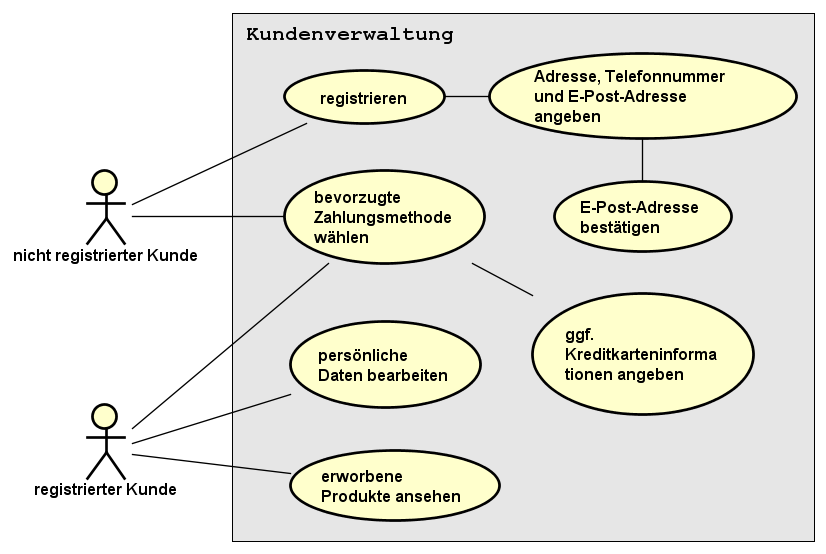
\includegraphics[width=0.8\textwidth]{szenario_kundenverwaltung.png}
\end{center}

Akteure: nicht registrierter \gls{Kunde}, registrierter \gls{Kunde}

Anwendungsfälle: Registrierung, persönliche Datenangabe, E-Post-Adressenbestätigung, Wahl der Zahlungsart, Kreditkarteninformationen angeben, persönliche Daten bearbeiten, erworbene Produkte ansehen 

Textuelle Beschreibung:

Ein noch nicht registrierter \gls{Kunde} kann sich registrieren indem er als erst seine persönlichen Daten angibt(Adresse, Telefonnummer, ect.). Als nächster Schritt muss er für eine vollständige Registrierung, seine E-Post-Adresse bestätigen. Wenn der neue \gls{Kunde} will, dann kann er seine bevorzugte Zahlungsmethode wählen. Nach dem Wählen der Zahlungsmethode, muss man im Fall der Kreditkartenabbuchung noch seine Kreditkarteninformationen angeben.
Ein bereits registrierter \gls{Kunde} kann immer seine bevorzugte Zahlungsart ändern oder wählen, seine persönliche Daten ändern oder anpassen und die von ihm schon erworbene Produkte ansehen. 


%
% % Automatisch generiertes Glossar
%
%\glsaddall % das sorgt dafür, dass alles Glossareinträge gedruckt werden, nicht nur die verwendeten. Das sollte nicht nötig sein!
\printglossaries
Siehe \url{https://en.wikibooks.org/wiki/LaTeX/Glossary}.

%
% % Glossareinträge
%
\newglossaryentry{Computer}
{
  name=Computer,
  description={Gerät zur Verarbeitung zur Daten, das die Daten einlesen, verarbeiten, speichern und ausgeben kann}
}

\newglossaryentry{Kunde}
{
	name=Kunde,
	plural=Kunden,
	description={(Zahlende) Benutzer des Onlineshops.}
}

\newglossaryentry{Plug-In}
{
	name=Plug-In,
	plural=Plug-Ins,
	description={Erweiterte Komponenten des iMage-Basic-Paket.}
}

\newglossaryentry{Sonderangebot}
{
	name=Sonderangebot,
	plural=Sonderangebote,
	description={Meist ein Produkt oder eine Zusammenstellung von mehreren Produkten, erhältlich für einen niedrigeren Preis als das normale Angebot.}
}

\newglossaryentry{upgraden}
{
	name=upgraden,
	description={beschreibt das Hinzufügen von weiteren Komponenten und das Verbessern eines bereits vorhandenen Grundbaustein.}
}

\newglossaryentry{Onlineshop}
{
	name=Onlineshop,
	plural=Onlineshops,
	description={Eine Plattform die es einem ermöglich mithilfe eines Internetzuganges Waren einzukaufen und anzusehen.}
}

\newglossaryentry{iMage}{
	name=iMage,
	description={Dabei handelt es sich um ein Bildbearbeitungsprogramm.}
}

\newglossaryentry{Bestaetigungsnachricht}
{
	name=Bestaetigungsnachricht,
	plural=Bestaetigungsnachrichten,
	description={eine Nachricht die meistens online verschickt wird, welche eine Link beinhaltet. Durch das ausführen des Links, kann man die Echtheit der Adresse bestätigen.}
}

\newglossaryentry{Browser}
{
	name=Browser,
	plural=Browsers,
	description={Eine Oberfläche die es einem \gls{Computer}nutzer ermöglicht Webseiten zu besuchen.}
}

\newglossaryentry{Opera}
{
	name=Opera,
	description={Opera ist ein kostenloser, auf einer quelloffenen Rendering-Engine basierender Webbrowser}
}

\newglossaryentry{Mozilla Firefox}
{
	name=Mozilla Firefox,
	description={Firefox ist ein freier Webbrowser des Mozilla-Projektes}
}

\newglossaryentry{Internet Explorer}
{
	name=Internet Explorer,
	description={Internet Explorer ist ein Webbrowser des Softwareherstellers Microsoft für dessen Betriebssystem Windows}
}

\newglossaryentry{Google Chrome}
{
	name=Google Chrome,
	description={Google Chrome ist ein Webbrowser des US-amerikanischen Unternehmens Google}
}

\newglossaryentry{Safari}
{
	name=Safrai,
	description={Safari ist ein Webbrowser des Unternehmens Apple. Er gehört zum Lieferumfang von Mac OS X ab der Version Mac OS X Panther sowie von iOS und ersetzte den vorher mitgelieferten Microsoft Internet Explorer für Mac als Standard-Browser.}
}
\end{document}
